% Energy level diagrams - illustrating Hund's rule
% Author: Henri Menke
\documentclass[tikz, border=10pt]{standalone}
\usepackage{siunitx}
\usetikzlibrary{shapes.callouts}
\tikzset{
  level/.style   = { ultra thick },
  connect/.style = { dashed, red },
  notice/.style  = { draw, rectangle callout, callout relative pointer={#1} },
  label/.style   = { text width=2cm },
  trans/.style   = { dashed, blue }
}
\begin{document}
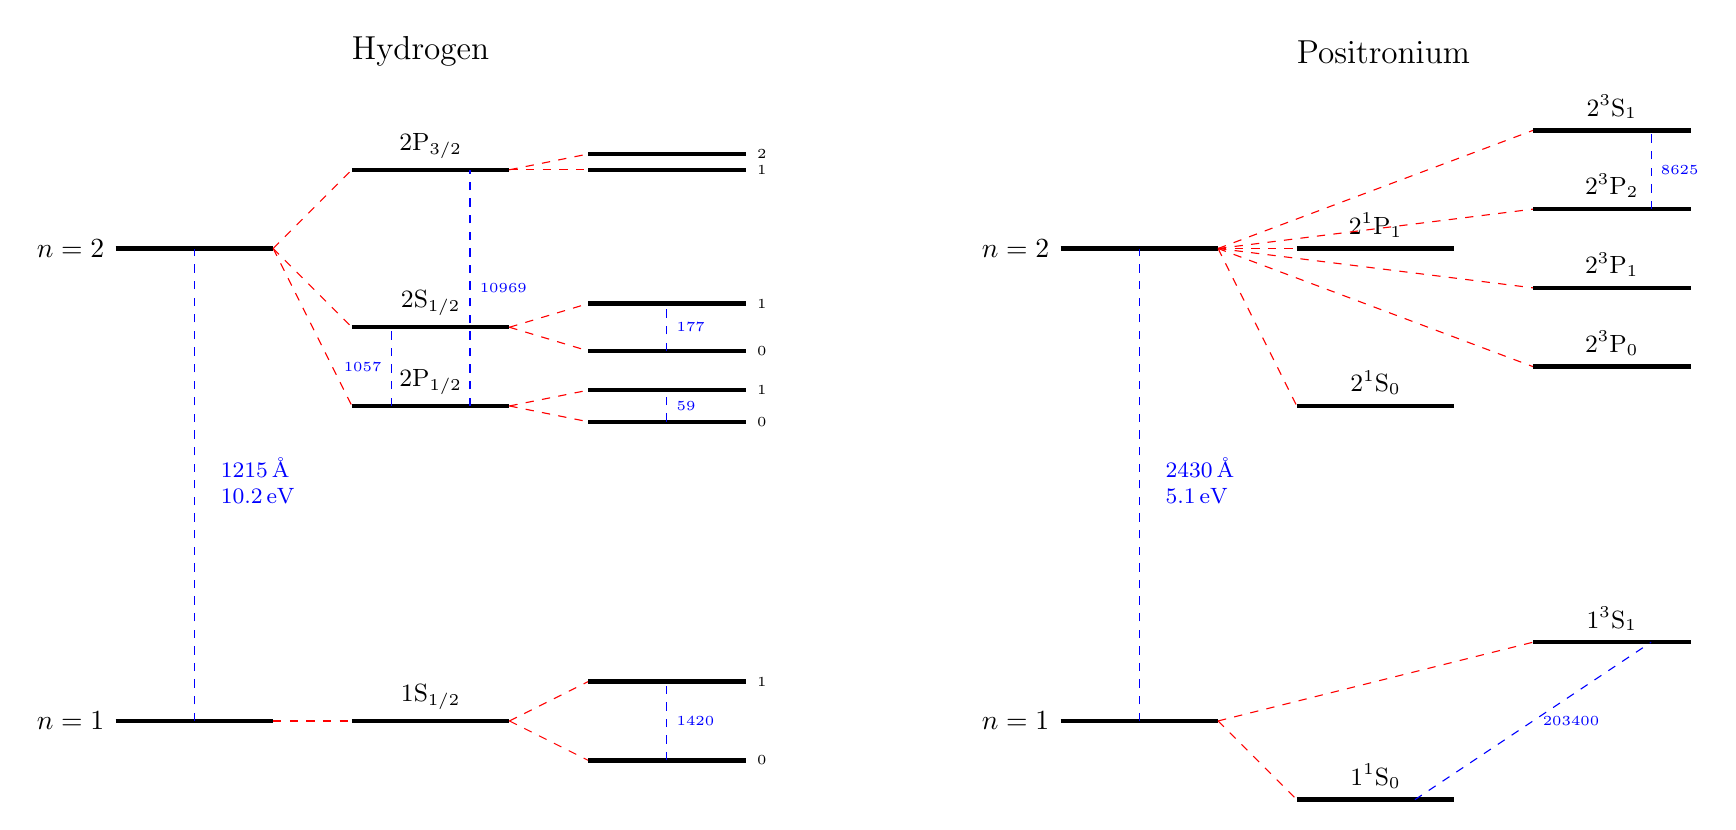
\begin{tikzpicture}
    \draw[level] node[left] at (0,0) {\( n=1 \)} (0,0) -- (2,0);
    \draw[level] node[left] at (0,6) {\( n=2 \)} (0,6) -- (2,6);

    \draw[level] (3,4) -- node[above] {\small2P$_{1/2}$} (5,4);
    \draw[level] (3,5) -- node[above] {\small2S$_{1/2}$} (5,5);
    \draw[level] (3,7) -- node[above] {\small2P$_{3/2}$} (5,7);

    \draw[level] (3,0) -- node[above] {\small1S$_{1/2}$} (5,0);

    \draw[connect] (2,6) -- (3,4);
    \draw[connect] (2,6) -- (3,5);
    \draw[connect] (2,6) -- (3,7);

    \draw[connect] (2,0) -- (3,0);

    \draw[connect] (5,7) -- (6,7)  ;
    \draw[connect] (5,7) -- (6,7.2);
    \draw[level] (6,7)   -- (8,7)   node[right] at (8,7)   {\tiny1};
    \draw[level] (6,7.2) -- (8,7.2) node[right] at (8,7.2) {\tiny2};

    \draw[connect] (5,5) -- (6,5.3);
    \draw[connect] (5,5) -- (6,4.7);
    \draw[level] (6,5.3) -- (8,5.3) node[right] at (8,5.3) {\tiny1};
    \draw[level] (6,4.7) -- (8,4.7) node[right] at (8,4.7) {\tiny0};

    \draw[connect] (5,4) -- (6,4.2);
    \draw[connect] (5,4) -- (6,3.8);
    \draw[level] (6,4.2) -- (8,4.2) node[right] at (8,4.2) {\tiny1};
    \draw[level] (6,3.8) -- (8,3.8) node[right] at (8,3.8) {\tiny0};

    \draw[connect] (5,0) -- (6,0.5) ;
    \draw[connect] (5,0) -- (6,-0.5);
    \draw[level] (6,0.5) -- (8,0.5)  node[right] at (8,0.5)  {\tiny1};
    \draw[level] (6,-0.5)-- (8,-0.5) node[right] at (8,-0.5) {\tiny0};

    \draw[trans] (1,0) -- node[right] {\footnotesize \begin{tabular}{l} $\SI{1215}{\angstrom}$\\$\SI{10.2}{eV}$\end{tabular}} (1,6);

    \draw[trans] (3.5,4) -- node[left]  {\tiny 1057} (3.5,5);
    \draw[trans] (4.5,4) -- node[right] {\tiny 10969} (4.5,7);

    \draw[trans] (7,-0.5) -- node[right] {\tiny 1420} (7,0.5);
    \draw[trans] (7,3.8)  -- node[right] {\tiny   59} (7,4.2);
    \draw[trans] (7, 4.7) -- node[right] {\tiny  177} (7,5.3);


    \node[label] at (4,8.5)  {\large Hydrogen};





    \draw[level] node[left] at (12,0) {\( n=1 \)} (12,0) -- (14,0);
    \draw[level] node[left] at (12,6) {\( n=2 \)} (12,6) -- (14,6);

    \draw[connect](14,0)  -- (15,-1) ;
    \draw[connect](14,0)  -- (18, 1) ;
    \draw[level] (15,-1)  -- node[above] {\small1$^1$S$_0$} (17,-1);
    \draw[level] (18, 1)  -- node[above] {\small1$^3$S$_1$} (20, 1);

    \draw[connect](14,6)  -- (15,6) ;
    \draw[connect](14,6)  -- (15,4) ;
    \draw[level] (15,6)   -- node[above] {\small2$^1$P$_1$} (17,6);
    \draw[level] (15,4)   -- node[above] {\small2$^1$S$_0$} (17,4);

    \draw[connect](14,6)  -- (18,4.5) ;
    \draw[connect](14,6)  -- (18,5.5) ;
    \draw[connect](14,6)  -- (18,6.5) ;
    \draw[connect](14,6)  -- (18,7.5) ;
    \draw[level] (18,7.5) -- node[above] {\small2$^3$S$_1$} (20,7.5);
    \draw[level] (18,6.5) -- node[above] {\small2$^3$P$_2$} (20,6.5);
    \draw[level] (18,5.5) -- node[above] {\small2$^3$P$_1$} (20,5.5);
    \draw[level] (18,4.5) -- node[above] {\small2$^3$P$_0$} (20,4.5);

    \draw[trans] (13,0) -- node[right] {\footnotesize \begin{tabular}{l} $\SI{2430}{\angstrom}$\\$\SI{5.1}{eV}$\end{tabular}} (13,6);

    \draw[trans] (16.5,-1)  -- node[right]  {\tiny 203400} (19.5,1);
    \draw[trans] (19.5,6.5) -- node[right]  {\tiny 8625}   (19.5,7.5);

    \node[label] at (16,8.5)  {\large Positronium};
  %% Draw labels
  %\node[label] at (4,5.5)  {Spin-spin interaction};
  %\node[label] at (7,5.5)  {Orbit-orbit interaction};
  %\node[label] at (10,5.5) {Spin-orbit interaction};
%
  %% Draw annotations
  %\node[notice={(0.5,0.5)}, text width=1.5cm] at (2,-3) {Hunds rule \# 1};
  %\node[notice={(0,1)}] at (4,-4) {Why is triplet lower};
  %\node[notice={(0.7,0.7)}, text width=3cm] at (6,-5)
%    {Why is higher angular momentum state lower energy?};
  %\node[notice={(-0.9,0.9)}, text width=1.5cm] at (9,-5) {Hunds rule \# 2};
  %\node[notice={(-0.2,1.6)}, text width=3cm] at (11,-6.5)
%    {Why is low total angular momentum state lower in energy?};
  %\node[notice={(-0.5,0.5)}, text width=1.5cm] at (12,-5) {Hunds rule \# 3};
\end{tikzpicture}
\end{document}
